\graphicspath{{../code/grid_pathfinding/data/plots/}}
% Babel en espanol rotula los cuadros flotantes como «Cuadro», pero el
% preambulo configura cleveref para que las referencias digan «Tabla». Se
% unifica aqui, que es un archivo propio, para no tocar preamble.tex.
\renewcommand{\tablename}{Tabla}

\subsection{Tiempo de ejecución}

La \Cref{fig:tiempo} y la \Cref{tab:grid_tiempos} resumen el tiempo de los tres
algoritmos sobre los doce tamaños del experimento. La separación entre
paradigmas es tan grande que solo se aprecia en escala logarítmica doble: en
$16 \times 16$, el mayor tamaño donde ambas soluciones exactas se ejecutan, la
fuerza bruta tarda $1{,}70$ segundos y la programación dinámica $8{,}4$
microsegundos, una razón superior a $2 \times 10^5$. La misma programación
dinámica resuelve la grilla de $1024 \times 2048$, con más de dos millones de
celdas, en $53$ milisegundos.

\begin{figure}[H]
  \centering
  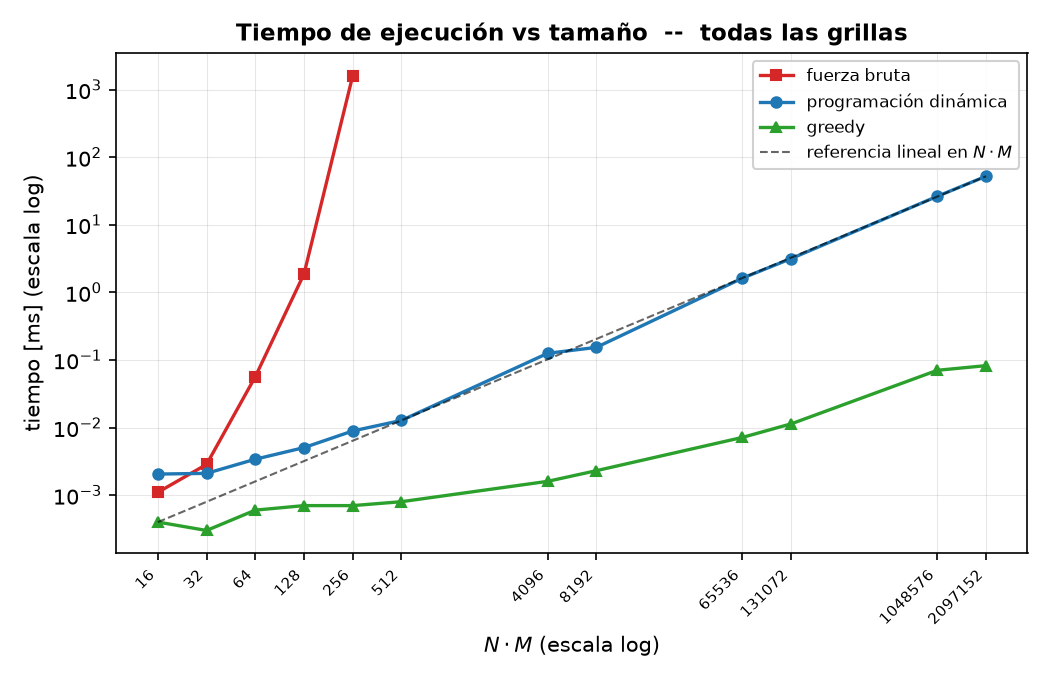
\includegraphics[width=0.62\textwidth]{tiempo_vs_tamano.png}
  \caption{Tiempo de ejecución contra área de la grilla, mediana de las tres
  repeticiones y las 24 instancias de cada tamaño. La recta punteada es una
  referencia lineal en $N \cdot M$; la programación dinámica se le ajusta desde
  las 4096 celdas. La fuerza bruta se interrumpe en 256 celdas porque el
  enunciado la limita a $N + M \leq 32$.}
  \label{fig:tiempo}
\end{figure}

% Generado automaticamente por grid_pathfinding/scripts/plot_generator.py
% NO EDITAR A MANO: se sobrescribe al correr 'make plots'.
\begin{table}[H]
\centering
\small
\begin{tabular}{lrrrr}
\hline
Grilla & Fuerza bruta & Dinámica & Greedy & Memoria DP \\
{} & [ms] & [ms] & [ms] & [KB] \\
\hline
$4 \times 4$ & 0.0011 & 0.0020 & 0.0004 & 0.4 \\
$4 \times 8$ & 0.0029 & 0.0021 & 0.0003 & 0.8 \\
$8 \times 8$ & 0.0565 & 0.0034 & 0.0006 & 1.7 \\
$8 \times 16$ & 1.8700 & 0.0051 & 0.0007 & 3.4 \\
$16 \times 16$ & 1602.9943 & 0.0089 & 0.0007 & 6.8 \\
$16 \times 32$ & -- & 0.0128 & 0.0008 & 13.5 \\
$64 \times 64$ & -- & 0.1254 & 0.0016 & 108.1 \\
$64 \times 128$ & -- & 0.1535 & 0.0023 & 216.2 \\
$256 \times 256$ & -- & 1.6238 & 0.0072 & 1728.5 \\
$256 \times 512$ & -- & 3.1616 & 0.0113 & 3456.8 \\
$1024 \times 1024$ & -- & 26.3895 & 0.0703 & 27650.0 \\
$1024 \times 2048$ & -- & 52.2726 & 0.0824 & 55299.0 \\
\hline
\end{tabular}
\caption{Tiempo (mediana de todas las repeticiones e instancias de cada tamaño) y memoria auxiliar de la programación dinámica. El guion indica que la fuerza bruta no se ejecuta por la cota $N+M \leq 32$.}
\label{tab:grid_tiempos}
\end{table}


Conviene precisar cuál es la cota de la fuerza bruta, porque la intuición
engaña. La cantidad de caminos de una grilla es $\binom{N+M-2}{N-1}$, que para
$16 \times 16$ son $155$ millones, pero el recorrido en profundidad no paga un
costo por camino sino por prefijo: cada nodo del árbol de estados es un prefijo
distinto, y la cantidad de prefijos que terminan en $(i,j)$ es
$\binom{i+j}{i}$. La suma de esos binomios sobre toda la grilla vale
exactamente $\binom{N+M}{N} - 1$, o sea $601$ millones de nodos para
$16 \times 16$, casi cuatro veces la cantidad de caminos. La diferencia está en
que el recorrido comparte los prefijos pero vuelve a caminar los
sufijos~\cite{algorithms_erickson}. La igualdad se comprobó contando los nodos
visitados sobre grillas libres de ocho tamaños distintos, y coincide en los
ocho.

El tipo de terreno afecta a la fuerza bruta en una dirección que vale la pena
notar: las murallas la \emph{abaratan}, porque cada una poda una rama completa
del árbol. Los $1{,}70$ segundos de la tabla agregan los cuatro tipos, pero
separados por terreno la mediana en $16 \times 16$ va de $3058$ milisegundos en
las grillas libres a $592$ en las de murallas y $628$ en las mixtas, un factor
de cinco. Las grillas con minas, en cambio, apenas bajan a $2622$
milisegundos, y la razón es exactamente la regla del problema: una mina no
bloquea el paso, solo cuesta blindaje, de modo que casi no poda el árbol de
estados. Solo las murallas lo podan. Comparar
\texttt{tiempo\_vs\_tamano\_murallas.png} con
\texttt{tiempo\_vs\_tamano\_libre.png} lo muestra con claridad.

\subsection{Contraste con las cotas teóricas}

Graficar el tiempo no basta para afirmar que una cota es la correcta. La
\Cref{fig:normalizado} divide el tiempo medido por la cota de cada algoritmo:
si el modelo de costo es el adecuado, la curva debe aplanarse en un valor
constante, que es el costo real por unidad de trabajo.

\begin{figure}[H]
  \centering
  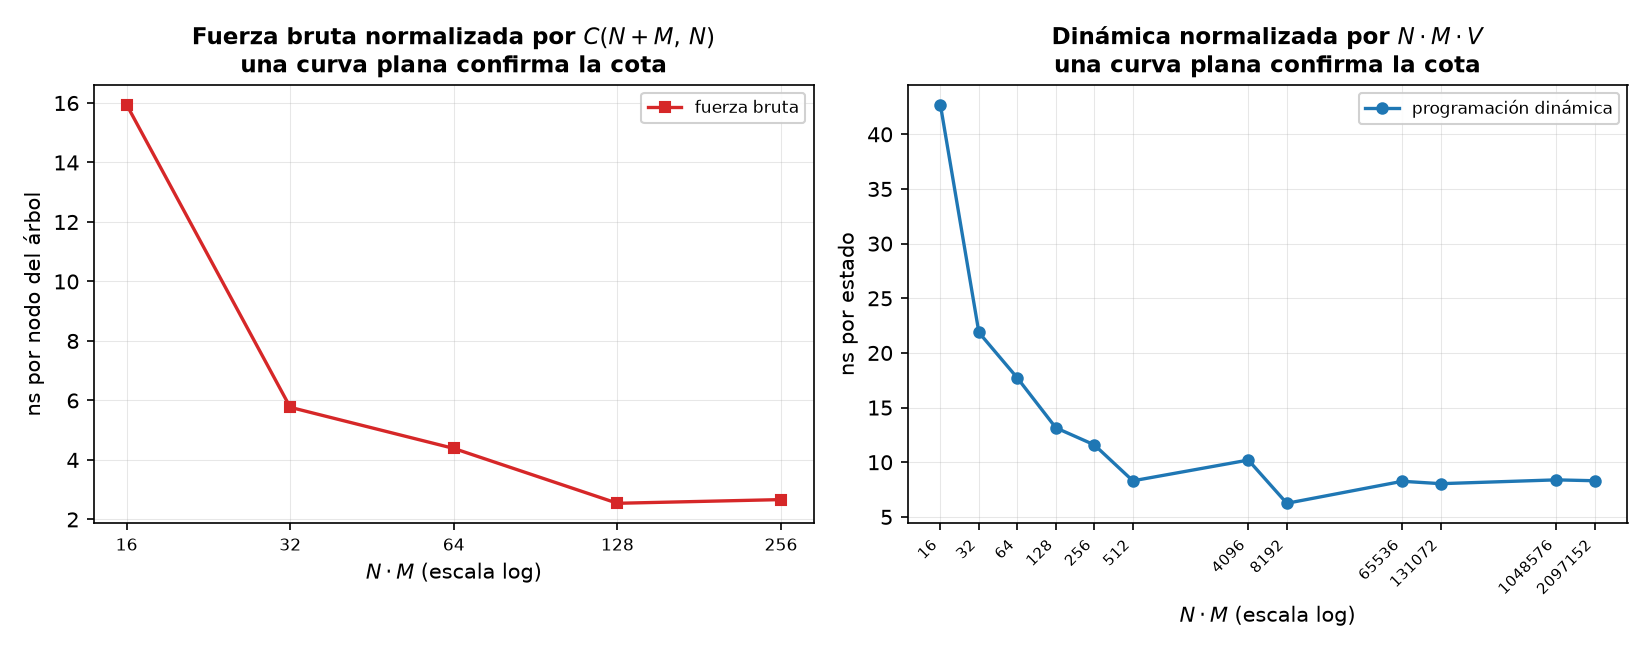
\includegraphics[width=0.88\textwidth]{normalizado_cotas.png}
  \caption{Tiempo normalizado por la cota teórica de cada algoritmo. A la
  izquierda la fuerza bruta dividida por $\binom{N+M}{N}$, a la derecha la
  programación dinámica dividida por $N \cdot M \cdot V$. Ambas se aplanan, lo
  que confirma que esos son los modelos de costo correctos.}
  \label{fig:normalizado}
\end{figure}

Las dos se aplanan. La fuerza bruta cae de $15{,}9$ a $2{,}6$ nanosegundos por
nodo y queda ahí desde las 128 celdas, y la programación dinámica cae de $50$ a
unos $8{,}5$ nanosegundos por estado, con todos los valores desde las 512
celdas contenidos entre $7{,}1$ y $10{,}2$.
La caída inicial de ambas no contradice la cota: es el costo fijo, que a esos
tamaños pesa más que el trabajo útil, porque una grilla de $4 \times 4$
resuelve 48 estados pero paga igual las reservas de memoria y la llamada a la
función. Estas dos mesetas son el resultado central del informe en lo que
respecta a tiempo, porque no solo miden sino que validan el modelo teórico de
cada paradigma.

\subsection{Uso de memoria}

La columna de memoria de la \Cref{tab:grid_tiempos} se duplica exactamente al
duplicarse el área de la grilla, que es $\Theta(N \cdot M \cdot V)$ sin margen
de ambigüedad: los $55\,299$ KB de la grilla mayor son sus $6\,291\,456$
estados a nueve bytes cada uno, ocho del puntaje y uno de la decisión que
permite reconstruir el camino.

El greedy ocupa entre $0{,}2$ y $6$ KB, que es el camino de salida y nada más,
o sea $\Theta(N+M)$. La fuerza bruta aparece en cero y conviene explicar por
qué: su costo espacial también es $\Theta(N+M)$, pero vive en la pila de
recursión, y el contador instrumenta el heap. No es un artefacto de medición
sino una propiedad del algoritmo, y en las instancias permitidas esa pila son a
lo más 32 marcos. La figura \texttt{memoria\_vs\_tamano.png} muestra las tres
curvas.

\subsection{Calidad de la solución greedy}

La heurística tiene dos formas de ser peor que el óptimo y conviene medirlas
por separado. La primera es fallar: quedarse sin celdas candidatas y no
alcanzar la meta, pese a que el generador garantiza que existe al menos un
camino válido. La \Cref{fig:falla} muestra que eso ocurre en 38 de las 288
instancias, un $13{,}2$ por ciento, y que está concentrado donde la regla
predice. De los 38 fracasos, 20 son de grillas con murallas y 17 de grillas
mixtas, contra uno solo en grillas con minas y ninguno en grillas libres, sobre
72 instancias de cada tipo. Es consistente con el protocolo: la única forma de
quedarse sin candidatas es que las dos celdas vecinas sean murallas, porque una
mina solo se descarta cuando queda una sola vida.

\begin{figure}[H]
  \centering
  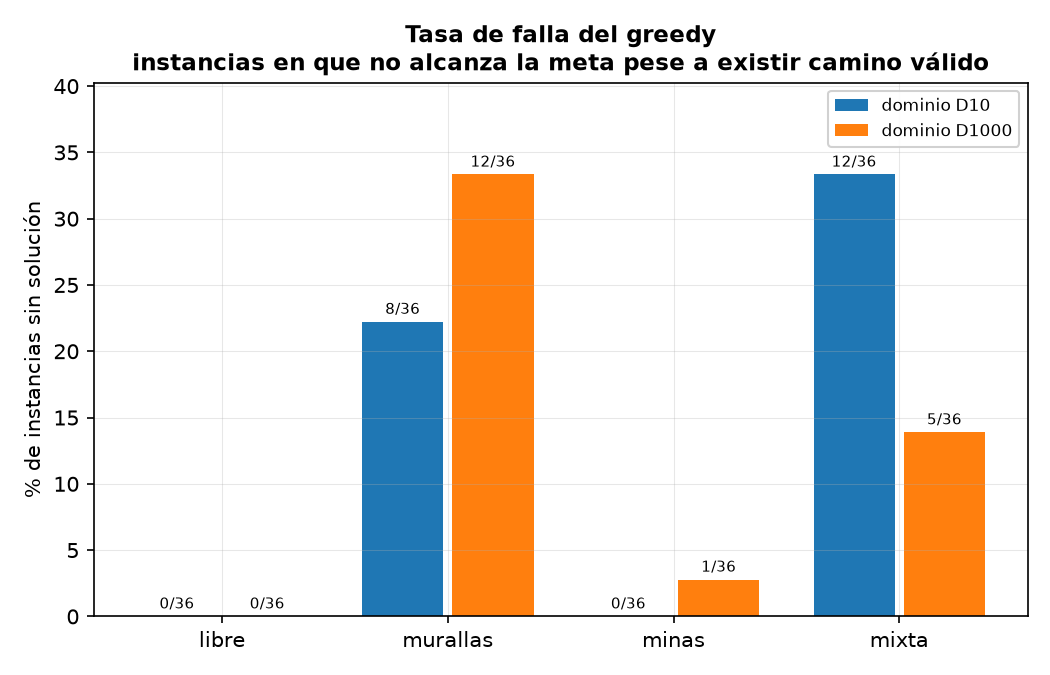
\includegraphics[width=0.60\textwidth]{tasa_falla_greedy.png}
  \caption{Proporción de instancias en que el greedy no alcanza la meta, por
  tipo de terreno y dominio. Las etiquetas indican los casos absolutos sobre el
  total de cada casilla.}
  \label{fig:falla}
\end{figure}

% Generado automaticamente por grid_pathfinding/scripts/plot_generator.py
% NO EDITAR A MANO: se sobrescribe al correr 'make plots'.
\begin{table}[H]
\centering
\small
\begin{tabular}{llrrrr}
\hline
Tipo & Dominio & Instancias & Sin solución & $\Delta$ mediana & $\Delta$ máxima \\
\hline
libre & D10 & 36 & 0 & 180 & 7417 \\
libre & D1000 & 36 & 0 & 12741 & 769946 \\
murallas & D10 & 36 & 8 & 114 & 7301 \\
murallas & D1000 & 36 & 12 & 19389 & 791288 \\
minas & D10 & 36 & 0 & 99 & 7834 \\
minas & D1000 & 36 & 1 & 14432 & 770790 \\
mixta & D10 & 36 & 12 & 96 & 6931 \\
mixta & D1000 & 36 & 5 & 9506 & 744092 \\
\hline
\end{tabular}
\caption{Calidad de la solución greedy. La brecha $\Delta = s(C^*) - s(C_{\text{greedy}})$ se calcula solo sobre las instancias en que la heurística alcanza la meta.}
\label{tab:grid_calidad}
\end{table}


La segunda forma de ser peor es llegar con menos puntaje, que es la brecha
$\Delta = s(C^{*}) - s(C_{\text{greedy}})$ de la \Cref{tab:grid_calidad}. Esa tabla hay
que leerla con cuidado, porque agrega seis tamaños cuyos caminos van de 6 a
3070 movimientos y la brecha crece con el largo del camino, de modo que la
comparación entre tipos queda dominada por el peso de cada tamaño. De hecho,
restringiendo el análisis a las grillas pequeñas el tipo murallas es el de
menor brecha, y con el conjunto completo pasa a ser el mayor: esa inversión es
un artefacto de la agregación y no un hallazgo sobre el terreno.

\begin{figure}[H]
  \centering
  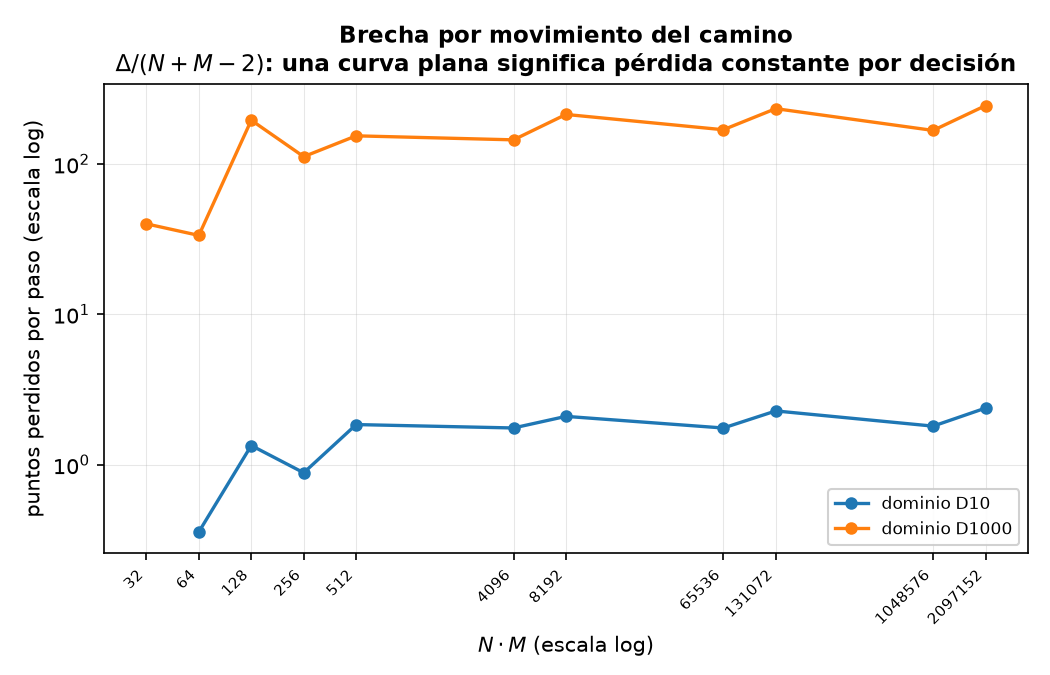
\includegraphics[width=0.60\textwidth]{brecha_por_paso.png}
  \caption{Brecha dividida por los $N+M-2$ movimientos del camino. La meseta
  indica que la heurística pierde una cantidad constante por decisión, y que su
  deterioro con el tamaño es acumulación y no degradación de la regla.}
  \label{fig:brechapaso}
\end{figure}

La forma correcta de responder cómo se degrada el greedy con el tamaño es
normalizar por la cantidad de decisiones que toma. La \Cref{fig:brechapaso}
divide la brecha por los $N+M-2$ movimientos del camino, y el resultado es una
meseta: en las instancias de 512 celdas o más, la mediana de la pérdida es de
$2{,}00$ puntos por paso en el dominio D10 y de $197{,}13$ en D1000. Es decir
que la regla no empeora al crecer la grilla, sino que acumula un error de
magnitud estable, y que $\Delta \approx c \cdot (N+M)$ con $c$ del orden de dos
puntos por movimiento en D10. La razón entre las dos mesetas es $98{,}6$, casi
exactamente la razón entre los dos dominios, lo que muestra que la heurística
se comporta igual a ambas escalas de valores una vez normalizada.

Normalizada de la misma forma, la brecha tampoco depende mucho del terreno: en
D10 la mediana por paso va de $1{,}80$ en las grillas con murallas a $2{,}18$
en las libres, y en D1000 de $172$ a $218$, un rango estrecho comparado con las
diferencias que sugería la \Cref{tab:grid_calidad} sin normalizar. La
conclusión es que el tipo de terreno decide sobre todo \emph{si} la heurística
llega a la meta, y mucho menos cuánto pierde por decisión cuando llega.

Eso explica de paso por qué el enunciado pide la brecha como resta y no como
cociente: con valores negativos o cero, $s(C_{\text{greedy}})/s(C^{*})$ no
tendría interpretación, y los puntajes tampoco son comparables entre dominios
porque $P$ vale lo mismo que la mejor celda posible de cada uno.
